\documentclass{beamer} 
\usepackage[utf8]{inputenc}
\usepackage[T1]{fontenc}

\usetheme{default}
\setbeamertemplate{navigation symbols}{}

\title{WIPS - Wireless Indoor Presence Sensing} 
\author{Erik Grafström, Max Morén, Erik Olsson} 
\date{May 31, 2011} 

\begin{document}

\begin{frame}
	\titlepage
\end{frame}

\begin{frame}
\frametitle{Scenario}
	
	\begin{figure}
		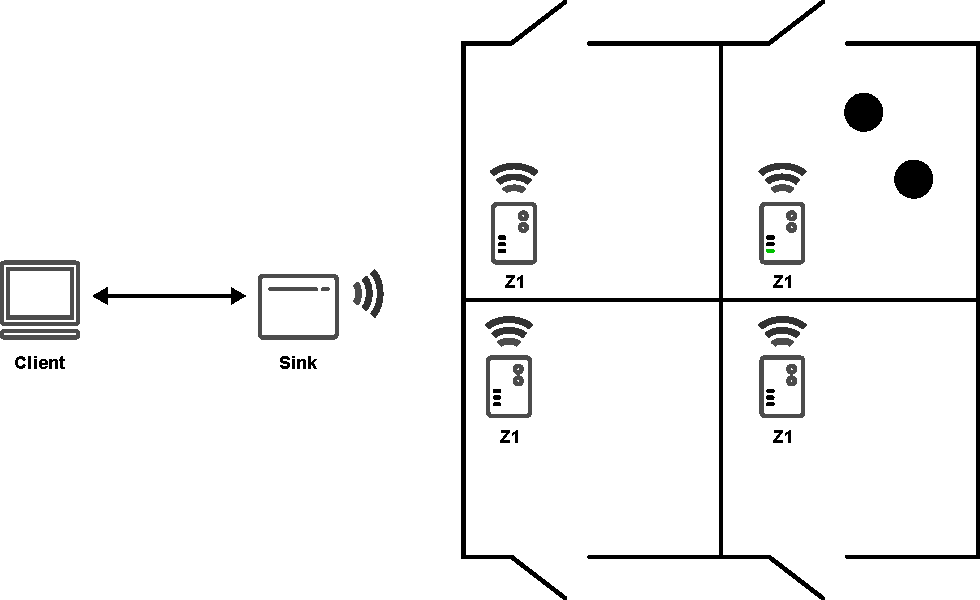
\includegraphics[width=\textwidth]{images/scenario.pdf}
		\caption{}
		\label{fig:scenario}
	\end{figure}
	
\end{frame}

\begin{frame}
\frametitle{Goals}

	\begin{block}

		\begin{itemize}

		\item
		
		Research existing WSN networking stacks and environmental monitoring techniques.
		\item
	Create and implement heuristics for indoor presence sensing.

		\item
	Evaluation of different networking solutions and energy efficient MAC protocols.
		\item
Implement and deploy working WSN based on evaluation results.
		\item
Implement data manager and web interface for data presentation.
		
		\end{itemize}

	\end{block}

\end{frame}

\begin{frame}
\frametitle{WSN hardware}

	\begin{columns}

		\column{0.5\textwidth}
	
			\begin{figure}
				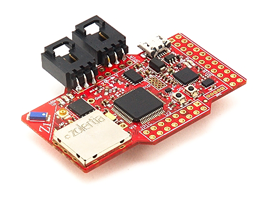
\includegraphics[width=0.5\textwidth]{images/z1.png}
				\caption{\url{http://zolertia.sourceforge.net/wiki/images/4/4f/Z1-B-medium.png}}
				\label{fig:z1}
			\end{figure}

		\column{0.5\textwidth}

			\begin{figure}
				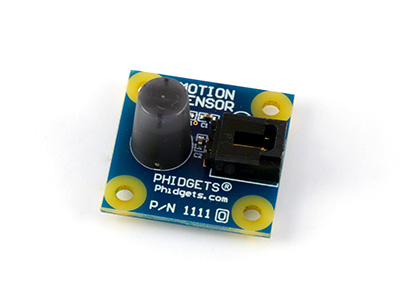
\includegraphics[width=0.5\textwidth]{images/1111.jpg}
				\caption{\url{http://www.phidgets.com/images/1111.jpg}}
				\label{fig:1111}
			\end{figure}

			\begin{figure}
				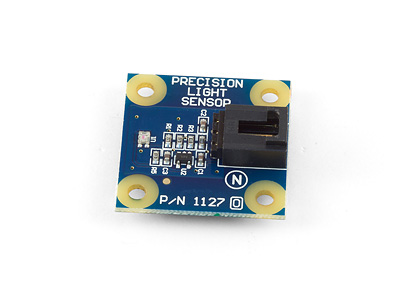
\includegraphics[width=0.5\textwidth]{images/1127.jpg}
				\caption{\url{http://www.phidgets.com/images/1127.jpg}}
				\label{fig:1127}
			\end{figure}

	\end{columns}

\end{frame}

\begin{frame}
\frametitle{Home automation hardware}

	\begin{columns}

		\column{0.5\textwidth}
	
		\begin{center}
			\begin{figure}
				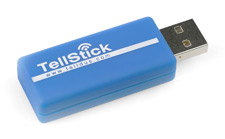
\includegraphics[width=0.5\textwidth]{images/tellstick.jpg}
				\caption{\url{http://www.evermedia.se/media/5984/tellstick.jpg}}
				\label{fig:tellstick}
			\end{figure}
		\end{center}

		\column{0.5\textwidth}

		\begin{center}
			\begin{figure}
				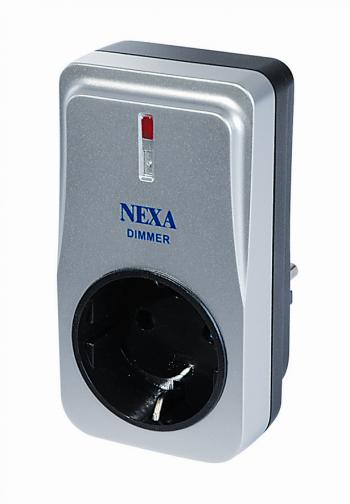
\includegraphics[width=0.5\textwidth]{images/lycr-300.jpg}
				\caption{\url{http://www.nexa.se/res/produktbilder_stora/lyc_dimmer.jpg}}
				\label{fig:lycr-300}
			\end{figure}
		\end{center}

	\end{columns}

\end{frame}

\begin{frame} 
\frametitle{Who we are}

	\begin{block}

		Erik Grafström

	\end{block}

	\begin{block}

		Max Morén
	
	\end{block}
	
	\begin{block}
	
		Erik Olsson

	\end{block}

\end{frame} 

\begin{frame}
\frametitle{Rime network stack}

	\begin{center}
		\begin{figure}
			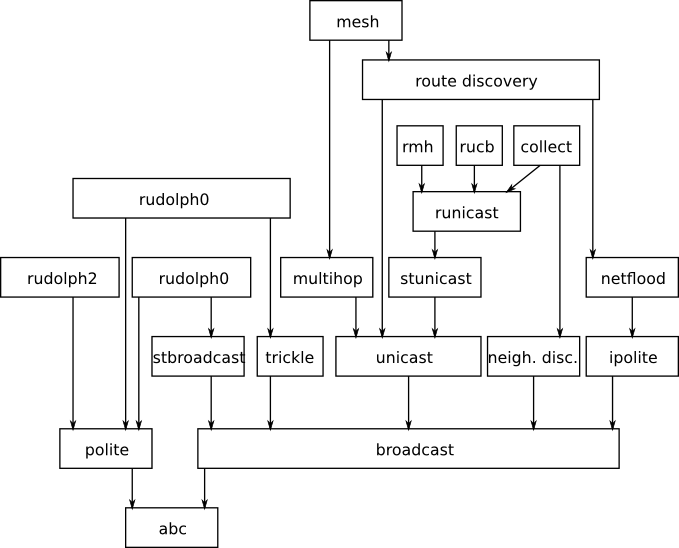
\includegraphics[width=0.75\textwidth]{images/rime.png}
			\caption{\url{http://senstools.gforge.inria.fr/lib/exe/fetch.php?cache=cache&media=os:contiki_rime.png}}
			\label{fig:rime}
		\end{figure}
	\end{center}

\end{frame}

\end{document}